% !TEX root = ../proj_report_outline.tex

\chapter{Evaluation of architectures}\label{C:exps}
In this chapter we present experimental results comparing the performance of the proposed architectures.
\hl{something something something}.

\section{Synthetic Tasks}
We first evaluate the performance of the architectures on some synthetic tasks. These tasks are designed
to be difficult and to exercise various faculties of the model.

\subsection{Addition}
\subsubsection{Task}
This task is designed to test the networks' ability to store information for long time periods. It first
featured in \autocite{Hochreiter1997}, although we use the slightly different formulation found more 
recently in \autocite{Le2015}. The problem is a common benchmark for RNNs and has featured in a number of
recent works (\autocite{Arjovsky2015, Henaff2016, Barone2016, Neyshabur2016} for example).

The inputs for this task are sequences of length \(T\). There are two inputs, one sampled from a uniform
distribution over the range \([0,1]\) while the other is zero except for two locations where it is one.
The location of the first one is always chosen to be earlier than \(T/2\) while the second is after.
The goal is to output at the last time step the sum of the two random values that were presented when the
second input was one. Pseudocode for an algorithm to generate sequences is presented in the appendix,
section~\ref{sec:additionpseudo}.
This task becomes harder as the \(T\) increases because the length of time the numbers have to
be remembered for increases.

\subsubsection{Experiment Setup}
We test a number of architectures on sequences with \(T\) of \(250, 500\) and \(750\). As we are
concerned purely with the ability of the networks to solve the task, we generate a new batch of
sequences at each step. All models were allowed \(8\) hidden units and trained on batches of \(8\)
data items to minimise the squared error between the output of the network at the final time step and
the target value. Updates were applied using ADAM \autocite{Kingma2014} with a base learning rate chosen
from \(\{0.1, 0.01, 0.001, 0.0001\}\) according to speed of convergence. For all runs, training continued
for \(2000\) updates. While some authors have found they require significantly more updates for success
with certain architectures (up to 10,000,000 in the case of \autocite{Le2015}) we found most successful
architectures so converge within 500 on most sequences.

While previously reported results for this task stop at \(T=750\), the most successful architectures still
converge rapidly to a solution at this stage. In order to more fully test their limits we increase
\(T\) to 1,000, 5,000 and 10,000. The same parameters were used but only the architectures tested that
were able to solve the task at \(T=750\) were applied to the tasks.

The models tested were the LSTM, GRU, IRNN \autocite{Le2015} and our TGU. We use a standard LSTM without
peephole connections. For the TGU we separate the bias matrices and use a layer of ReLUs for the candidate
production.

\subsubsection{Results}
The baseline result for this task is a squared error of \(0.1767\) which corresponds to predicting
\(1\) for every input. Many architectures are unable to perform significantly better than this.



\subsection{Variable Binding}
This task is designed to test the architectures' ability to store arbitrary patterns in memory and
associate them with a label. We term this ``variable binding'' as to solve the task the network needs
to be capable of associating an arbitrary value with a specific label. This task is a natural
sub-problem of many large scale problem domains to which RNNs have already been successfully applied.
An example is translation -- in an end-to-end translation system, the network must perform tasks such
as detecting subjects and objects of sentences, store them appropriately and reproduce them at an
arbitrary time. \hl{can we cite gmarcus and say that humans tend to prefer identity mappings, so maybe
our nets should (when trying to do things humans are good at eg language)?}

Curiously, we could
not find a satisfactory task in the literature which exercised this ability.
Close alternatives include
the copy task in \autocite{Hochreiter1997} and the variants considered in \autocite{Graves2014}, but these
are concerned with recalling the order in which symbols arrive. The ``variable assignment'' task
used to evaluate the Associative LSTM \autocite{Danihelka2016} has the same aim in mind, but it is more
complex as the assignment and retrieval instructions are spread over multiple time steps.


\subsubsection{Task}
We propose the following synthetic task to exercise the ability of the network to store and retrieve
arbitrary patterns: inputs and targets are sequences of length \(T\). Inputs at each time step are
binary vectors of size \(D+N\). The first \(D\) elements of the input are the ``pattern bits'' while
the remaining \(N\) are the ``label bits''. \(N\) different binary patterns are presented to the
network at randomly chosen time steps in the first half of the sequence, the pattern bits are zero at
all other times. Immediately before a pattern is presented, one of the label bits is set. The label
bit is then held until a randomly chosen time step where it is cleared.
At this point, the network must output the corresponding pattern. Label bits are never reused. The target
sequence to match consists of vectors of size \(D\), containing the appropriate pattern at the moment each
of the label bits switches off and zeros elsewhere. Figure~\ref{fig:vbinddata} shows example input/target
pairs for various \(N\) (best viewed without antialiasing), 
while algorithm~\ref{alg:vbinddata} in the appendix demonstrates how to produce appropriate data.

\begin{figure}
\centering
	\begin{tabu} to \textwidth {XX}
		Input & Target \\
		
\includegraphics[width=0.45\textwidth, interpolate=false]{exps/vbind/100x1input} & 
		
\includegraphics[width=0.45\textwidth, interpolate=false]{exps/vbind/100x1target} \\
		
\includegraphics[width=0.45\textwidth, interpolate=false]{exps/vbind/100x2input} & 
		
\includegraphics[width=0.45\textwidth, interpolate=false]{exps/vbind/100x2target} \\
		
\includegraphics[width=0.45\textwidth, interpolate=false]{exps/vbind/100x3input} & 
		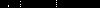
\includegraphics[width=0.45\textwidth, interpolate=false]{exps/vbind/100x3target} \\
	\end{tabu}
	\caption[Example instances of variable binding]{Example input/target pairs for the three
	different variable binding tasks. All have length 100, with 8 bit patterns -- all that differs
	is the number of patterns the network may have to remember at once.}
	\label{fig:vbinddata}
\end{figure}

\begin{figure}
\centering
	\begin{tabu} to \textwidth {XX}
		Input & Target \\
		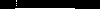
\includegraphics[width=0.45\textwidth, interpolate=false]{exps/vbind/100x1tguinput} & 
		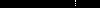
\includegraphics[width=0.45\textwidth, interpolate=false]{exps/vbind/100x1tguoutput} \\
		
\includegraphics[width=0.45\textwidth, interpolate=false]{exps/vbind/100x2tguinput} & 
		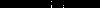
\includegraphics[width=0.45\textwidth, interpolate=false]{exps/vbind/100x2tguoutput} \\
		
\includegraphics[width=0.45\textwidth, interpolate=false]{exps/vbind/100x3tguinput} & 
		
\includegraphics[width=0.45\textwidth, interpolate=false]{exps/vbind/100x3tguoutput} \\
	\end{tabu}
	\caption[Example successful outputs for variable binding]{Outputs from TGU models that that
	achieved good results.}
	\label{fid:vbindcorrect}
\end{figure}

\begin{figure}
\centering
	\begin{tabu} to \textwidth {XX}
		Input & Target \\
		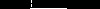
\includegraphics[width=0.45\textwidth, interpolate=false]{exps/vbind/100x1gruinput} & 
		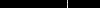
\includegraphics[width=0.45\textwidth, interpolate=false]{exps/vbind/100x1gruoutput} \\
		
\includegraphics[width=0.45\textwidth, interpolate=false]{exps/vbind/100x2gruinput} & 
		
\includegraphics[width=0.45\textwidth, interpolate=false]{exps/vbind/100x2gruoutput} \\
		
\includegraphics[width=0.45\textwidth, interpolate=false]{exps/vbind/100x3gruinput} & 
		
\includegraphics[width=0.45\textwidth, interpolate=false]{exps/vbind/100x3gruoutput} \\
	\end{tabu}
	\caption[Example of baseline for variable binding]{Output from GRUs demonstrating the baseline
	behaviour -- the timing is correct but the output is not related to the input.}
	\label{fig:vbindfail}
\end{figure}

This task involves a number of interesting concepts. A correct solution will need to learn a
transformation from input patterns to hidden states and then learn the inverse transform
to produce the correct output. The requirement of invertibility suggests a strong reason
for the success of the TGU with linear candidate updates, as the correct output can be reconstructed
by applying the inverse affine transformation. \hl{we ensure overspecified, because learning identities is hard?}

Storing and recalling multiple distinct items also requires the ability to be selective about
updating the hidden state.\hl{gates are good for this}

\subsubsection{Experiment Setup}
For this task we found the same hyper parameters to be the best for all models
(that is to say, grid search was unable to find any with demonstrably better performance).
Models were trained with a batch size of \(32\) using ADAM with a base learning rate of \(0.01\).
We ceased training after 5000 steps --  although some models were only just beginning to learn
by this time, it is sufficient to see the difference in how easily they are able to arrive
at a solution.

As the targets are binary vectors we use a sigmoid output layer and train to minimise the
sum of the cross entropy at each output at each time step.
For all results reported we use eight bit patterns and test on sequences of length 100, 200 and 500
with one, two and three patterns leading to nine different experiments.

The baseline behaviour which all architectures (including the Vanilla RNN) achieved rapidly
is to wait until any of the label bits turns off and output a pattern with mean 0.5. Guessing
0.5 (or randomly with probability 0.5) achieves a cross entropy of \(-\log 0.5 = 0.69315\), so
this will achieve a total loss on sequences with \(N\) eight bit patterns of \(-8N\log 0.5\).
Examples of a networks exhibiting this behaviour can be found in table~\ref{fig:vbindfail}.

As the aim is to assess the ability of the networks to solve the task, we train in an online
fashion. This means that rather than generate a training and test set, we generate new sequences
as required and only report the training error as in this case it is equivalent to generalisation
performance.

We set the number of hidden units to ten times the number patterns to remember for each architecture.
This leads to considerable difference in the number of parameters, but this task is primarily
concerned with the ability of an RNN to use its memory sensibly, so it is fairest to ensure they
all have the same amount of memory. As the patterns are all eight bits, have ten hidden units
per pattern ensures it is possible for the networks to store the inputs directly and still have
a couple of units to track the state of the label bits. As the patterns are binary, it is very
easy for the networks to also learn a compressed representation, but we decided not to force them
into this behaviour to keep the task focused.

\subsubsection{Results}
We report results for the LSTM, GRU, IRNN and TGU. For the TGU we incorporate the biases into
the decomposition (we denote this TGU-C) and use linear activations. This was found to give the
most consistent results. We also tested the Vanilla RNN, which was unable to beat the baseline in
any tests and several TGU variants -- for clarity we only present the results of architectures which
showed at least some promise. We were unable to reliably train IRNNs on sequences longer than
100, despite heavy gradient clipping the gradients
consistently exploding leading to numerical instability. Due to this we only report IRNN results on
the tasks with sequence length 100.

While results were consistent, the training curves are very noisy -- this is a very difficult task
and none of the models are completely immune to the various problems that plague RNNs in general.
To obtain a clearer picture, we plot the median of five runs.

This task becomes harder both with increased length and more patterns to remember. Increasing the
length increases the length of time patterns must be remembered without degrading as well as
increasing the likelihood of vanishing gradients interfering with training. Increasing the number
of patterns to remember means that the RNN must learn to utilise its states in significantly more
complex ways.

\begin{figure}[p]
\begin{subfigure}[t]{0.3\linewidth}
	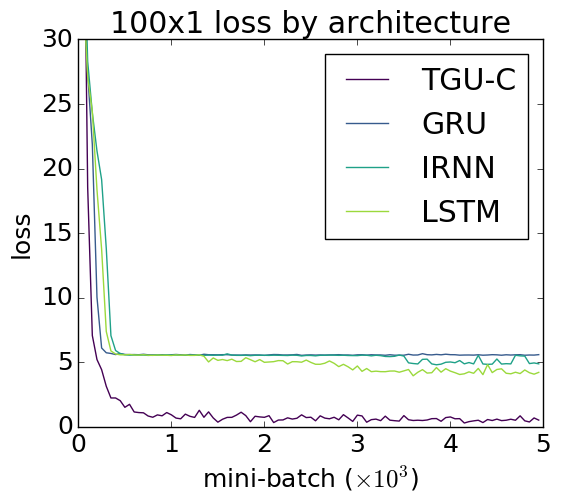
\includegraphics[width=\linewidth]{exps/vbind/plots/100x1}
	\caption{Sequence length 100.}
\end{subfigure}~
\begin{subfigure}[t]{0.3\linewidth}
	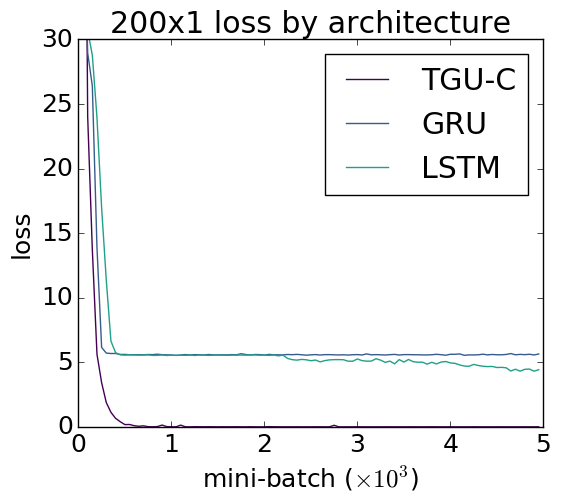
\includegraphics[width=\linewidth]{exps/vbind/plots/200x1}
	\caption{Sequence length 200.}
\end{subfigure}~
\begin{subfigure}[t]{0.3\linewidth}
	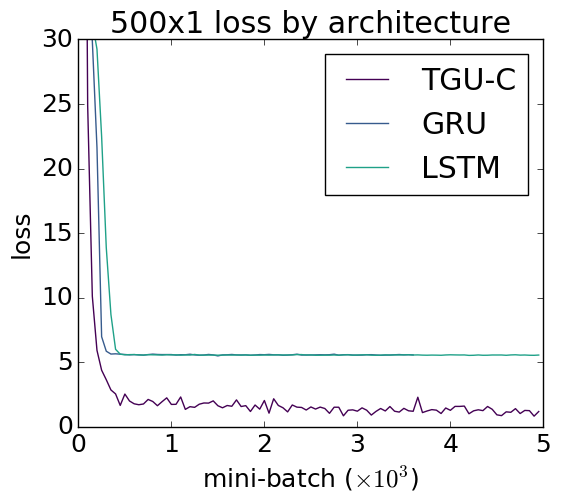
\includegraphics[width=\linewidth]{exps/vbind/plots/500x1}
	\caption{Sequence length 500.}
\end{subfigure}

\caption[Variable binding results, one pattern]
{Variable binding results for sequences containing \(1\) pattern to remember. The baseline loss for this
task is 5.5452.}
\label{fig:vbindn1}
\end{figure}

\begin{figure}[p]
\begin{subfigure}[t]{0.3\linewidth}
	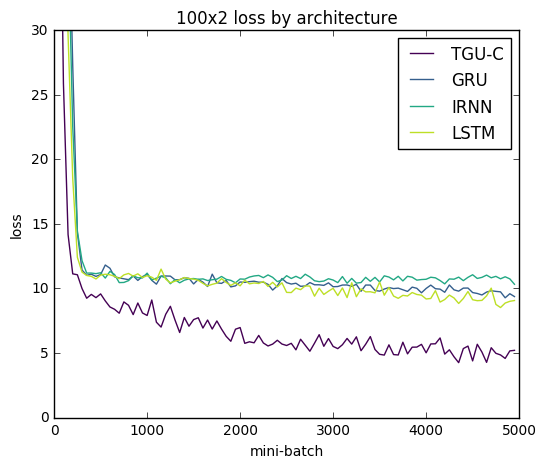
\includegraphics[width=\linewidth]{exps/vbind/plots/100x2}
	\caption{Sequence length 100.}
\end{subfigure}~
\begin{subfigure}[t]{0.3\linewidth}
	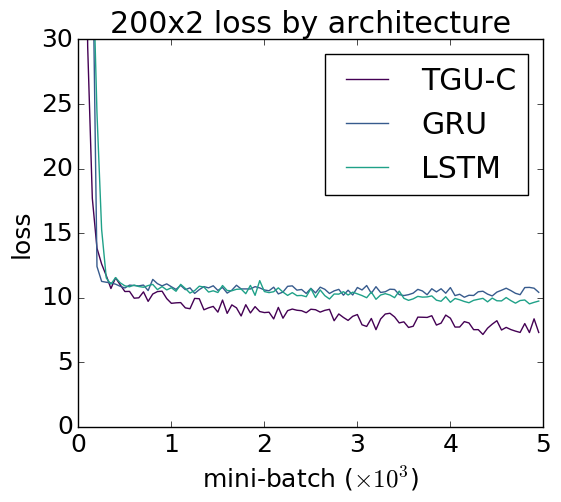
\includegraphics[width=\linewidth]{exps/vbind/plots/200x2}
	\caption{Sequence length 200.}
\end{subfigure}~
\begin{subfigure}[t]{0.3\linewidth}
	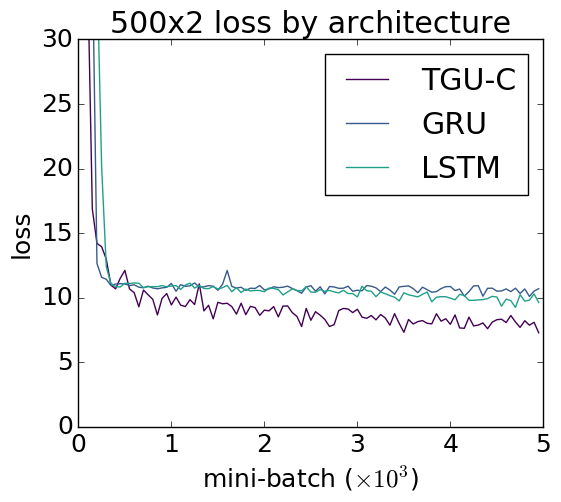
\includegraphics[width=\linewidth]{exps/vbind/plots/500x2}
	\caption{Sequence length 500.}
\end{subfigure}

\caption[Variable binding results, two patterns]
{Variable binding results for sequences containing \(2\) patterns to remember. The baseline loss for this
task is 11.0904.}
\label{fig:vbindn2}
\end{figure}

\begin{figure}[p]
\begin{subfigure}[t]{0.3\linewidth}
	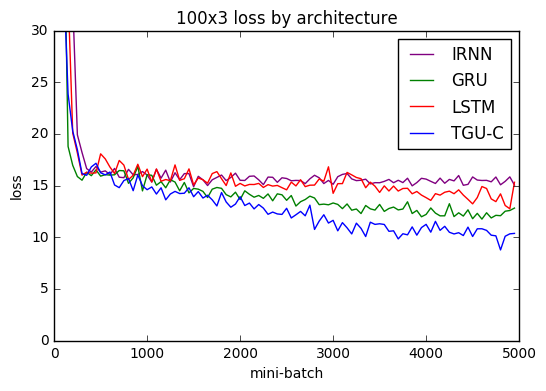
\includegraphics[width=\linewidth]{exps/vbind/plots/100x3}
	\caption{Sequence length 100.}
\end{subfigure}~
\begin{subfigure}[t]{0.3\linewidth}
	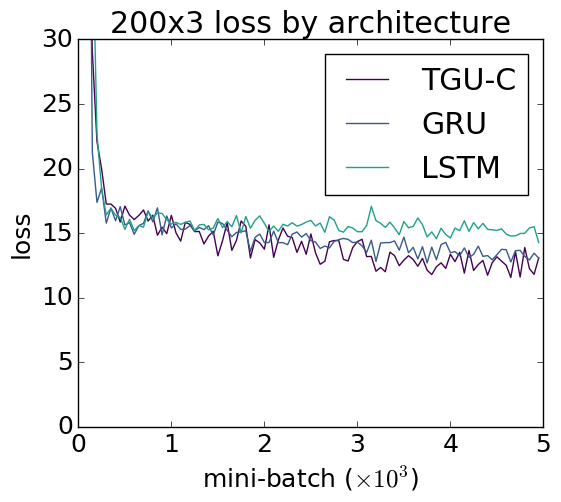
\includegraphics[width=\linewidth]{exps/vbind/plots/200x3}
	\caption{Sequence length 200.}
\end{subfigure}~
\begin{subfigure}[t]{0.3\linewidth}
	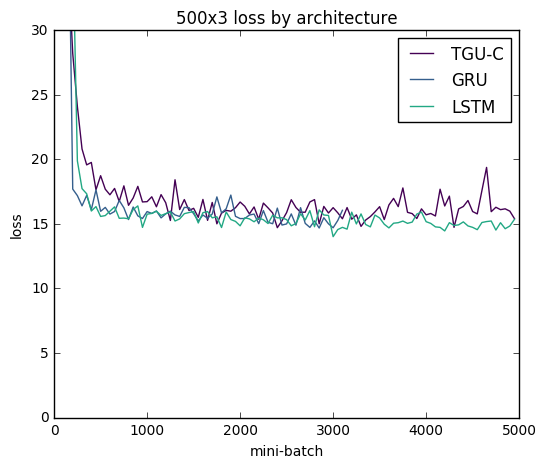
\includegraphics[width=\linewidth]{exps/vbind/plots/500x3}
	\caption{Sequence length 500.}
\end{subfigure}

\caption[Variable binding results, three patterns]
{Variable binding results for sequences containing \(3\) patterns to remember. The baseline loss for this
task is 16.6355.}
\label{fig:vbindn3}
\end{figure}

With only a single pattern to remember, the TGU dramatically outperformed the other
architectures. The LSTM was the most consistent of the other architectures tested,
although in every test by the time it had begun to escape from the baseline the TGU
had already converged. The GRU was able to make surprisingly little progress on this
task.

Increasing the number of items to remember, even just to two, appears to make the
task considerably more difficult. This perhaps highlights an issue with the manner
in which RNNs interact with their memory -- they are forced to attend to it all
at once. If we consider a TGU-style RNN in which the candidate state does not
depend on the previous hidden states, it must learn a redundant mapping to embed
the input into the state-space. This is because it can not rely on the label
bits to determine which of the two inputs it is processing (this would require
access to the hidden states to determine which has switched on recently). If we
assume different sets of hidden states are used to represent inputs with different
associated labels, then the candidate update must propose to update both of them
with the new input and it is up to the gate to select which update to apply.
This seems like a perfectly reasonable solution, although learning such a redundant
mapping is going to be considerably more challenging than simply learning the single
reversible transformation required to solve the task when only a single pattern
is to be remembered. 

While LSTMs and GRUs are capable of this behaviour as well as more complex solutions,
the TGU is consistently able to outperform them, except on the hardest of the tasks.
We suggest that restricting the number of possible solution mechanisms in this way
helps the TGU find such solutions.

With two patterns to remember the TGU still makes the most progress 
below the baseline in the time allotted.
On the longer sequences progress is limited and none of the architectures
are close to converging although the TGU is the only architecture to
make notable progress.

When the number of patterns is increased to three all the architectures struggle.
With a sequence length of 100, there is some separation -- the TGU makes the most
progress although the GRU and LSTM also begin to progress beyond the baseline.
On the longer sequences, there is less of a clear result and when the sequence
length is up to 500, no models were capable of surpassing the baseline even when
allowed to train for significantly longer than reported in figure~\ref{fig:vbindn3}.

These results affirm that the TGU is competitive with the state of the art approaches.
They also suggest that the fundamental change -- focusing the expressive power in the
gate rather than the candidate update -- is not misguided and makes a fundamental
difference to the manner in which the network attends to its state.


\subsection{Sequential MNIST}
\hl{edit to reflect we only care about pmnist?}
A pair of recently proposed tasks which have gathered significant popularity lately
are based around attempting to classify the MNIST handwritten image dataset 
\autocite{Lecun1998}. To turn two dimensional images into a sequence task they are
flattened in one of two ways: either in scan-line order beginning from the top-left
going one row at a time or simply by taking a random permutation \autocite{Le2015}.

This gives two tasks in which the input is a one dimensional time series to be
classified. The MNIST digits are 28 by 28 digits, so the input sequences are
784 steps long. As the majority of the pixels are black with the activity focused
in the central region, the majority of the information in the scan-line version
is focused in the middle. Contrastingly, taking a random permutation of the indices
is highly likely to induce very long time dependencies, in addition to removing
any temporal correlations in the sequence by destroying the morphology. Consequently
the permuted version is significantly more challenging.

Although this has been widely used recently to benchmark architectural
advances in RNNs (see, for example 
\autocite{Zhang2016, Barone2016, Gao2016, Neyshabur2016, Cooijmans2016}
just from 2016), we argue that it does not necessarily provide a useful test of
a model's capabilities. We show this by achieving excellent performance
on the more challenging permuted task with a models which fail miserably
in real world applications. 

This is achieved by exploiting the fact
that although the permutation introduces artificially long time dependencies
the underlying data is very simple -- a simple k-Nearest Neighbour classifier
achieves 95\% accuracy \autocite{Lecun1998}. Combining the simplicity of the
class boundaries with the sparsity of the representation in pixel-space and we
can see that it should be possible to succeed simply by accumulating information
at each time step, building a compressed representation which is then classified
at the final time step.

\subsubsection{Proposed Architecture}
We propose an architecture specifically for this task which is a variant on
GMRNN proposed earlier, modified to allow for direct accumulation.
Further, we enforce this accumulative behaviour by applying a linear rectifier
to the state update. The hidden states are computed by:
\begin{equation}\label{eq:cpplus}
	\vec{h}_t = \vec{h}_{t-1} + \rho\left( \tran{\vec{x}}_t\tensor{W}\vec{h}_{t-1} + \mat{U}\vec{x}_t + \vec{b}\right).
\end{equation} This architecture should fail -- the gradients are almost
guaranteed to explode during back-propagation by the argument in section~\ref{sec:additive},
it can never remove information from its states (the state updates must be non-negative).
The only way it can make a context-dependent decision to ignore certain inputs is
if the tensor product is able to outweigh the rest of the calculation before the
non-linearity and force it to be negative. As we implement the tensor product
using a tensor in the CP decomposition, we refer to this architecture as the
``CP+''.

Despite its clear shortcomings, this model achieves remarkable success on the
sequential MNIST tasks. As discussed above we believe this is due to shortcomings
with the task rather than special properties of the above model, as the above
model is clearly very limited.

A model which seems slightly less absurd allows \emph{subtractive} forgetting:
\begin{align}\label{eq:cpdelta}
	\vec{a}_t &= \rho\left(\tran{\tilde{\vec{x}}}_t\widetilde{\tensor{W}}_a\tilde{\vec{y}}\right)\\
	\vec{b}_t &= \rho\left(\tran{\tilde{\vec{x}}}_t\widetilde{\tensor{W}}_b\tilde{\vec{y}}\right)\\
	\vec{h}_t &= \vec{h}_{t-1} + \vec{a}_t - \vec{b}_t.
\end{align} We denote this architecture ``CP-\(\Delta\)'' and consider only the variant in
which the bias matrices are incorporated into the tensor decomposition to keep the number
of parameters comparable. It appears more sensible
than the CP+ as it at least allows for the possibility of a negative state update.
However, this model will suffer from the same gradient issues as the CP+, although
they might be expected to be less pronounced as the negative term may
mollify the back-propagated error. In practice, we find this is not the case and
the model requires at least as much guidance as the CP+.

To enable training of this model we re-parameterise the weight matrices with a
form of \emph{weight normalisation} \autocite{Salimans2016a}. Typical
weight normalisation learns unconstrained weights but applies a differentiable
normalisation transformation before use. Salimans and Kingma normalise each
row of the weight matrices to have an \(l2\) norm of \(1\), we achieved
best results by dividing each matrix by its Frobenius norm.\footnote{
For a \(n \times m\) matrix \(\mat{U}\), the Frobenius norm is
\(||\mat{U}||_F = \sqrt{\sum_i^n\sum_j^mU_{ij}^2} = ||\vect(\mat{U})||_2\).}
Back-propagation proceeds as usual through the transformation.

\subsubsection{Experiments}
We are primarily concerned with the permuted task, although we report some
on the less challenging ordering as well to indicate that our models are
performing near the state-of-the-art on these tasks. Learning rate and rank
were found using grid-search. We train using ADAM with a batch size of 100.
for nearly all models, severe gradient clipping \autocite{Pascanu2013} is
required to train successfully, the best value was also found using grid
search.

Following \autocite{Le2015} all models tested have a single hidden layer of 100 units.
We use a grid search to find the best rank for the tensor models.

\subsubsection{Results}

\begin{figure}
\begin{subfigure}[t]{0.45\textwidth}
	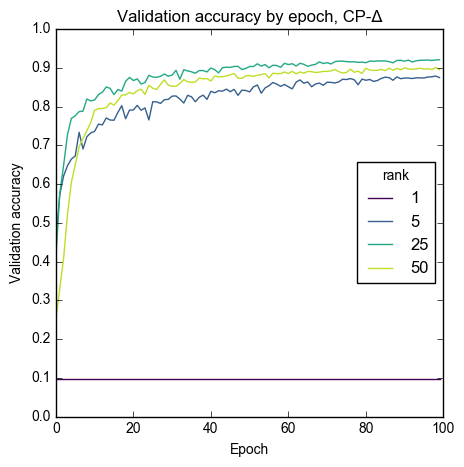
\includegraphics[width=\textwidth]{exps/mnist/cp-del-rank}
	\caption{CP-\(\Delta\) by rank}
\end{subfigure}~
\begin{subfigure}[t]{0.45\textwidth}
	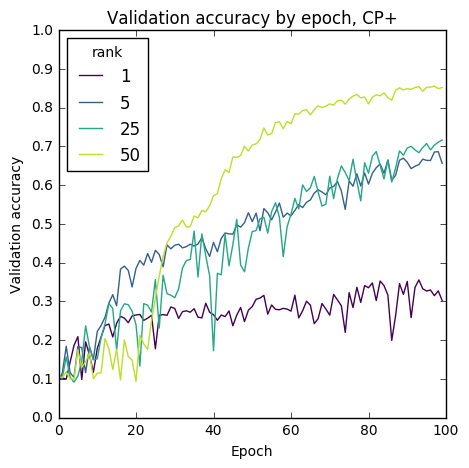
\includegraphics[width=\textwidth]{exps/mnist/cp+rank}
	\caption{CP+ by rank}
	\label{fig:cp+rank}
\end{subfigure}\\
\begin{subfigure}[t]{0.45\textwidth}
	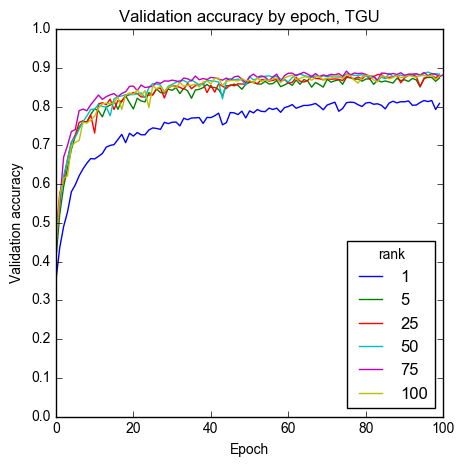
\includegraphics[width=\textwidth]{exps/mnist/tgurank}
	\caption{TGU by rank}
\end{subfigure}
\begin{subfigure}[t]{0.45\textwidth}
	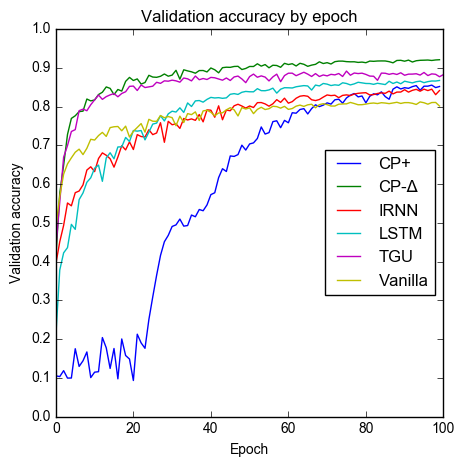
\includegraphics[width=\textwidth]{exps/mnist/allarchs}
	\caption{All architectures}
\end{subfigure}

\caption[Permuted MNIST results]{Performance (classification accuracy, \%)
 on the validation set of permuted MNIST
by rank of tensor decomposition.}
\label{fig:pmnistrank}
\end{figure}

\begin{table}

\begin{tabu} to \textwidth {r|l}
Architecture & Test Accuracy (\%)\\
\hline
TGU & 88.2\\
CP+ & 84.7\\
CP-\(\Delta\) & 91.5\\
IRNN (ours) & 84.0\\
LSTM (ours) & 86.3\\
Vanilla (ours) & 79.3\\
\hline
\emph{i}RNN \autocite{Le2015} & 82.0 \\
\emph{u}RNN \autocite{Arjovsky2015} & 91.4 \\
\emph{s}TANH-RNN \autocite{Zhang2016} & 94.0 \\
BN-LSTM \autocite{Cooijmans2016} &\textbf{95.4}\\
\hline
\end{tabu}

\caption{Test accuracy for permuted sequential MNIST.}
\label{tab:pmnist}
\end{table}

Final test accuracy for the best models on the permuted task
 is reported in table~\ref{tab:pmnist}. On the simpler version
all of the interesting models achieve between 97 and 99 per cent,
so we do not report further results as there are no insights to be
gained. Table~\ref{tab:pmnist} also includes recent results, all
of which were state-of-the-art for couple of months. Our models sit
in the middle of this range of results. 
This is remarkable as the 
best performing architecture, the CP-\(\Delta\) has fundamental
design flaws which cause it to fail on any other dataset we attempted
to train it on.

Figure~\ref{fig:pmnist} shows how the performance scales with rank of
the tensor decomposition. As the CP-\(\Delta\) incorporates the
bias matrices into the decomposition, reducing the rank should greatly
affect performance. Indeed, with a rank 1 decomposition the model is
incapable of learning anything. What is more curious is that the
best performing model is not the highest rank. These models are not
enormous, but the largest still have up to 40,000 parameters so it is
possible that the lower rank provides a regularising effect which helps
the model learn a more general solution.

The absurdity of the CP+ unit is clear from figure~\ref{fig:co+rank}.
It trains in an incredibly volatile fashion. Interestingly for ranks
1 and 50 the best parameters found by grid search included a gradient
threshold of 10, ten times the threshold needed for the other models.
As rank 50 achieved the best performance, this appears to be an
example of the benefits of operating at the ``edge of chaos'',
right on the edge between vanishing and exploding gradients and states
\autocite{Bertschinger2004}. Further, that the rank 1 model learns
at all is remarkable. The tensor product is this unit is severely
restricted, the vast majority of its learning power resides in a
feed-forward connection. This goes some way to affirming our suspicions
about this task -- although  it exhibits long time dependencies, the
benefit of using detailed contextual information at each time step is
limited.

\section{Real-world Data}
We now move on to more realistic datasets. All of the following tasks are
\emph{next-step prediction} tasks -- the goal of the network is to estimate
the probability of the next item in the sequence given the sequence so far:
\begin{equation} \label{eq:seqprob}
	p(\vec{x}_{t+1} | \vec{x}_{1},\ldots,\vec{x}_{t}).
\end{equation} The output layer of the RNN then has the task of converting
the hidden states into probabilities and so requires an appropriate non-linearity.
Training proceeds by maximising the log-likelihood of the data producing the
correct distribution.

Essentially this means that the target sequence is the input
sequence shifted across by one. If we prepend a special \emph{start-of-sequence}
symbol to the data sequence and append an \emph{end-of-sequence} symbol,
then the inputs to the network are simply all but the \emph{end-of-sequence}
and the outputs are all but the \emph{start-of-sequence}.

The end result is a statistical model of the sequence. We can sample from it
by simply feeding it the \emph{start-of-sequence} character and then repeatedly
sampling from the distribution generated by the current hidden states and
feeding the sample back in to the network. This can be an interesting way to
produce novel sequences \autocite{Graves2013}.

In all cases the data is split into three sets: training, test and validation.
The size of the splits vary as we attempt to remain consistent with prior work.
The validation set is used to monitor generalisation performance and to stop
training when the model begins to overfit to the training data. The manner in
which this is realised is by checking the average negative log-likelihood the model
achieves after each epoch of training. If the validation performance has improved,
we save a checkpoint containing the model parameters. After having trained for
a fixed number of epochs the best saved model is loaded and its performance is
evaluated on the test set.

The aim of this section is not to achieve state-of-the-art performance on
large datasets using enormous networks. Rather we seek to ascertain whether the
theoretical reasoning and intuitions developed in the preceding chapters hold
in a more realistic setting. \hl{some nice way to say this?? but the idea is
that we don't want to compete with hacks but to see if the ideas and guiding
principles we came up with are indeed sensible and to see whether our RNNs are
competitive in a restricted setting on smaller data without fancy engineering
tricks.}

\subsection{Polyphonic Music}
This task, introduced to the neural network community by 
\autocite{Boulanger-Lewandowski2012} consists of modelling four datasets of
polyphonic music. 



\subsubsection{Task}



\subsubsection{Experiments}
The four datasets are:
\begin{itemize}
\item[Pianomidi] {
	is a collection of classical piano scores originally sourced from
	\url{http://piano-midi.de}. We split the data according to
	\autocite{Poliner2007}. This data uses the full range of the piano,
	there are 88 distinct notes present although the polyphony is limited
	as the pieces must all be played by a human.}
\item[Nottingham] {
	is a set of folk tunes converted to MIDI by 
	\autocite{Boulanger-Lewandowski2012},\footnote{
	The originals are available at: \url{http://ifdo.ca/~seymour/nottingham/nottingham.html}}
	we use their split of the data. These tunes have the simplest structure and are
	generally quite short although they span a range of 63 distinct notes.}
\item[Muse] {
	comes originally from \url{http://www.musedata.org} and contains both orchestral and
	piano classical music. This dataset has a range of 84 distinct notes and due to the
	orchestral nature of many of the scores the polyphony can be quite high. Again we
	split the data according to \autocite{Boulanger-Lewandowski2012}.}
\item[JSB] {
	consists of all 382 chorales harmonised by J. S. Bach. This dataset has some of the
	lowest polyphony, at most four notes at once, although it is very consistent by its
	nature. This dataset also has the smallest range with a final range of 54 notes.
	We use the split of the data given in \autocite{Allan2004}.}
\end{itemize}

The data is converted from MIDI files (which contain note on/off events) to
an appropriate format by sampling the notes present at regular time intervals.
This gives binary vectors in which each element indicates with a one or a zero whether
a particular note is active or not.\footnote{Appropriately pre-processed data can
be downloaded from \url{http://www-etud.iro.umontreal.ca/~boulanni/icml2012}
courtesy of Boulanger-Lewandowski et al. \autocite{Boulanger-Lewandowski2012}.}
For each dataset, we fix the size of these vectors to the range of notes present in the
dataset (after transposing to C major or C minor, equivalent to centering the data).
\hl{point out that this is sensible, we aren't just being different for kicks}

Previous work is somewhat inconsistent with the size of these vectors. Of those that
report it, \autocite{Boulanger-Lewandowski2012} fix the size of the vectors for all
datasets to the range of 88 notes available on a piano while \autocite{Chung2014}
end up with much larger vectors although it is not clear why. In general this means
results can not be directly compared although it is worth noting they are similar,
with nearly all of our RNNs surpassing \autocite{Chung2014} and achieving performance
similar to the RNNs evaluated in \autocite{Boulanger-Lewandowski2012}. Given the differences
in setup, we would expect our RNNs to fare slightly worse as using larger data vectors
means many of the output units are redundant and never used. The network should learn this
quite quickly which will bring the average negative log-likelihood down.

All networks used a single hidden layer. The number of hidden nodes and the rank of
the tensor decomposition was chosen so that each network would have as close to
20,000 parameters when applied to the JSB dataset as possible. This was done to help
make the comparison more fair so that the comparison is not skewed by models such as
the LSTM which have a large number of parameters per hidden unit. The rank was set as
either \(1\) or a multiple of the hidden states, chosen from \(\{1/2, 1, 2\}\).
Table~\ref{tab:jsbsizes} shows the number of hidden units and the rank of the tensor
decomposition for the models evaluated. The networks used a sigmoid output layer to
appropriately model the fact that the multiple output units may need to be on at once.

\begin{table}
\begin{tabu} to \linewidth {r||c|c|c|c}
\hline
Model & \multicolumn{4}{|c}{hidden units/rank (parameters)} \\
\hline
Vanilla & \multicolumn{4}{|c}{96  (19927)} \\
LSTM & \multicolumn{4}{|c}{44 (20075)} \\
GRU & \multicolumn{4}{|c}{52 (19763)} \\
\hline
GMRNN & 95/1 (19870) & 71/35 (19872) & 58/58 (19775) & 45/90 (20125) \\
GMRNN-C & 349/1 (20005) & 106/52 (20142) & 76/76 (20119) & 53/106 (20248) \\
TGU &  80/1 (20030) & 63/31 (20156) &  53/53 (20248) & 41/82 (19817) \\
TGU-C &  176/1 (20000) & 88/44 (20075) & 66/66 (19855) & 48/96 (20071)\\
\hline
\end{tabu}
\caption[Model sizes for polyphonic music task]{Size of models for polyphonic music
modelling. Architectures with -C appended have the bias matrices combined with the
decomposition. Parameters are reported for inputs of size \(54\) as per the JSB dataset.
Rank is only reported if applicable.}
\label{tab:jsbsizes}
\end{table}

A preliminary grid search was undertaken on a subset of the architectures to determine
sensible ranges for the final experiments. Models reported were trained using ADAM with
a grid search over the following hyper-parameters: base learning rate from \(\{0.01, 0.001\}\),
maximum length of back-propagation through time chosen from \(\{75, 100\}\) steps
and rank chosen from the options in table~\ref{tab:jsbsizes}. Note that to keep the number
of parameters constant, changing the rank necessitates changing the number of hidden units
as well. The batch size was set to \(8\). For nearly all architectures best performance was
achieved with the lower learning rate while the best maximum length seemed to be more task-dependent.

\subsubsection{Results}
\begin{table}
\begin{tabu} to \linewidth {r||c|c|c}
\hline
		 \multicolumn{4}{c}{Nottingham} \\
    	& \emph{Train}      & \emph{Valid}    & \emph{Test} \\
\hline
Vanilla   & \textbf{3.3278} & 3.8680 & \textbf{3.8871}      \\ % sl 100
LSTM      & 3.5826          & 3.9683          & 4.0124		\\ % sl 100
GRU		  & 3.5876		    & 3.9871		  & 4.0157		\\ % sl 100
GMRNN	  & 3.3940		    & \textbf{3.8472} & 3.9055		\\ % rankone sl 100
GMRNN-C   & 3.7902		    & 4.1242          & 4.1350		\\ % rankhalf sl 75
TGU		  & 3.9652		    & 4.2069          & 4.2140		\\ % rankone sl100
TGU-C     & 4.0035		    & 4.2332	      & 4.2531		\\ % rankfull sl100
lin-TGU   & 3.9387		    & 4.2095	      & 4.2255		\\ % rankone sl 75
lin-TGU-C & 3.9927		    & 4.2726          & 4.2907\\ % rankhalf sl 100
\hline\hline
 \multicolumn{4}{c}{JSB} \\
    	& \emph{Train} & \emph{Valid} & \emph{Test} \\
\hline
Vanilla   & 8.0284	        & 8.5417	      & 8.6381   \\ % sl 75
LSTM      & 8.2058	        & 8.5444	      & 8.6633   \\ % sl 75
GRU		  & 8.1689	        & 8.5657	      & 8.6027   \\ % sl 75
GMRNN	  & 8.0526	        & 8.5465	      & 8.6084   \\ % rankone sl 75
GMRNN-C   & 8.0093	        & \textbf{8.4656} & 8.5369   \\ % rankhalf sl 100
TGU		  & \textbf{7.9357} & 8.5140	      & 8.6060   \\ % rankhalf sl 75
TGU-C     & 7.9731	        & 8.4926	      & \textbf{8.5307}   \\ % rankone sl 100
lin-TGU   & 8.0645	        & 8.7126	      & 8.7282   \\ % rankhalf sl 75
lin-TGU-C & 8.2257	        & 8.6549	      & 8.7117   \\ % rankhalf sl 100
\hline\hline
 \multicolumn{4}{c}{Pianomidi} \\
    	& \emph{Train} & \emph{Valid} & \emph{Test} \\
\hline
Vanilla   & 7.3874	        & 8.5956	      & 7.8093   \\ % sl 75
LSTM      & 7.3730	        & \textbf{8.5329} & 7.7542   \\ % sl 75
GRU		  & 7.3039	        & 8.5671	      & 7.7652   \\ % sl 100
GMRNN	  & 7.3598	        & 8.5890	      & 7.7676   \\ % rankone sl 100
GMRNN-C   & 7.4244	        & 8.7350	      & 7.8615   \\ % rankhalf sl 100
TGU		  & \textbf{7.2132} & 8.5981	      & 7.7161   \\ % rankhalf sl 100
TGU-C     & 7.2748	        & 8.5382	      & \textbf{7.7003}  \\ % rankhalf sl 75
lin-TGU   & 7.2866	        & 8.5807	      & 7.7475   \\ % rankhalf sl 75
lin-TGU-C & 7.3216	        & 8.5716	      & 7.7209   \\ % rankhalf sl 75
\hline\hline
 \multicolumn{4}{c}{Muse} \\
    	& \emph{Train} & \emph{Valid} & \emph{Test} \\
\hline
Vanilla   & 6.8954	        & 7.2597	      & 7.3619   \\ % sl 100
LSTM      & 7.0777	        & 7.3652	      & 7.4159   \\ % sl 75
GRU		  & 7.0001	        & 7.3256	      & 7.3824   \\ % sl 100
GMRNN	  & \textbf{6.8864} & \textbf{7.2089} & \textbf{7.3089}   \\ % rankone sl 100
GMRNN-C   & 6.9135	        & 7.3349	      & 7.4296   \\ % rankfull sl 100
TGU		  & 7.4524	        & 7.7076	      & 7.6879   \\ % rankone sl 100
TGU-C     & 7.4551	        & 7.6842	      & 7.6719   \\ % rankhalf sl 100
lin-TGU   & 7.5478	        & 7.7732	      & 7.7428   \\ % rankhalf sl 75
lin-TGU-C & 7.6134	        & 7.8147	      & 7.7949   \\ % rankfull sl 75
\hline
\end{tabu}

\caption[Polyphonic music modelling results]
{Results on polyphonic music datasets. Numbers are average negative log-likelihood, lower is better.
 ``-C'' appended to the tensor units indicates the bias matrices are folded into the decomposition,
 otherwise they are separate. ``lin-'' appended to the start of the TGUs indicates that they
 use no non-linearity on the candidate state update.}
\label{tab:jsbresults}
\end{table}

Results for the four datasets are found in table~\ref{tab:jsbresults}. We report the average
negative log-likelihood the best early-stopped models assign the data vectors over
the training, test and validation sets.

In general the tensor units performed better than their counterparts except on
Nottingham, the simplest of the datasets. This dataset consists of folk songs which
are often very formulaic in their harmony. Correspondingly, simple models seem to be able to
perform very well. It also seems to be the case that there is something about the structure
of the data which suits the Vanilla RNN -- the best GMRNN (which was the closest to the
Vanilla RNN out of all architectures) had a rank \(1\) tensor decomposition. This means
that it was functionally nearly identical to a Vanilla RNN.

\subsection{PTB}
\subsection{War and Peace}